\section{Descrição}

O projeto de unidade (PU) tem como objetivo a implementação de um sistema \fuzzy para se saber a umidade do solo adequada para cada período (Germinação, Crescimento, Floração e Maturação) de um  determinado tipo de plantação. Isso se deve ao motivo que cada planta possui as suas próprias características, como o tipo de raiz, o seu coeficiente de crescimento, capacidade de sobreviver a um determinado período sem a quantidade de água adequada.    


\begin{figure}[h!]
\centering
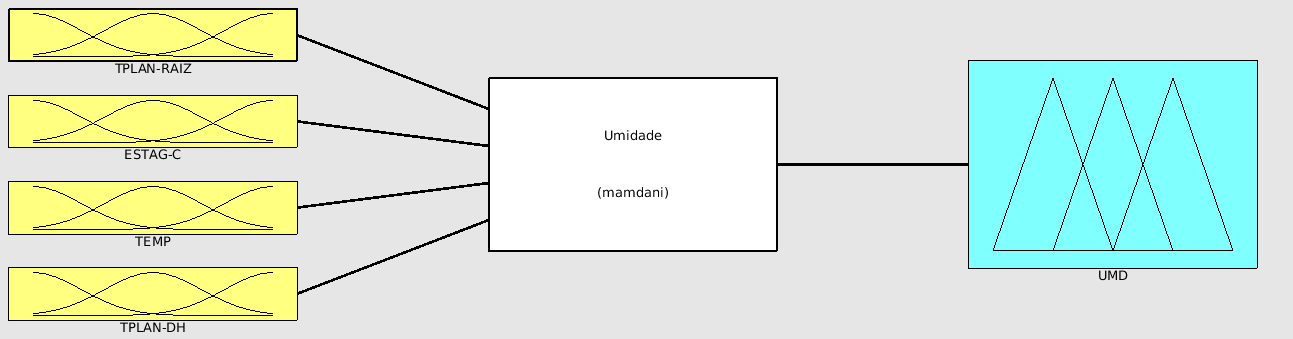
\includegraphics[width=1\linewidth]{Descricao/Imagens/Sistema}
\caption{Sistema \fuzzy}
\label{fig:Sistema}
\end{figure}


\subsection{Variáveis do Sistema - Variáveis de entrada}

As variáveis de entradas utilizadas foram: 

\begin{itemize}
	\item TPLAN-RAIZ (tipo-de-planta-raiz);
	\item TPLAN-DH (tipo-de-planta-déficit-hídrico);
	\item ESTAG-C (estágio-de-crescimento-da-planta);
	\item TEMP (temperatura)
\end{itemize}

\newpage
\subsubsection{TPLAN-RAIZ}

\textbf{TPLAN-RAIZ (TIPO-DE-PLANTA-RAIZ):} Essa variável está associada à profundidade do sistema radicular da planta no solo, ou, à Profundidade Efetiva das raízes da planta onde se concentram 80\% de suas raízes. Quanto maior a profundidade das raízes, maior a
necessidade de dotação hídrica.

\begin{table}[h!]
	\centering
	\rowcolors{1}{}{lightgray}
	\caption{Profundidade efetiva das raízes}
	\label{tab:TPLAN-RAIZ}
	\begin{tabular}{lcc}
		\hline \hline
		\textbf{Cultura}                 & \textbf{Gomes (1994)} & \textbf{Pires et al. (1999)} \\
		\hline
		Abacaxi                 & 30-60        & 20-70               \\
		Hortaliças (ex. alface) & 20-40        & 10-15               \\
		Arroz                   & -            & 10-25               \\
		Algodão                 & 80-180       & 30                  \\
		Cana-de-açúcar          & 50-100       & 70                  \\
		Cítricos (ex. laranja)  & 90-150       & 60                  \\
		Melancia                & 100-150      & -                   \\
		Melão                   & 70-100       & -                   \\
		Milho                   & 60-120       & 40                  \\
		Morango                 & -            & 30                  \\
		Tomate                  & 60-120       & 50                  \\
		\hline
	\end{tabular}
\end{table}


\begin{figure}[h!]
\centering
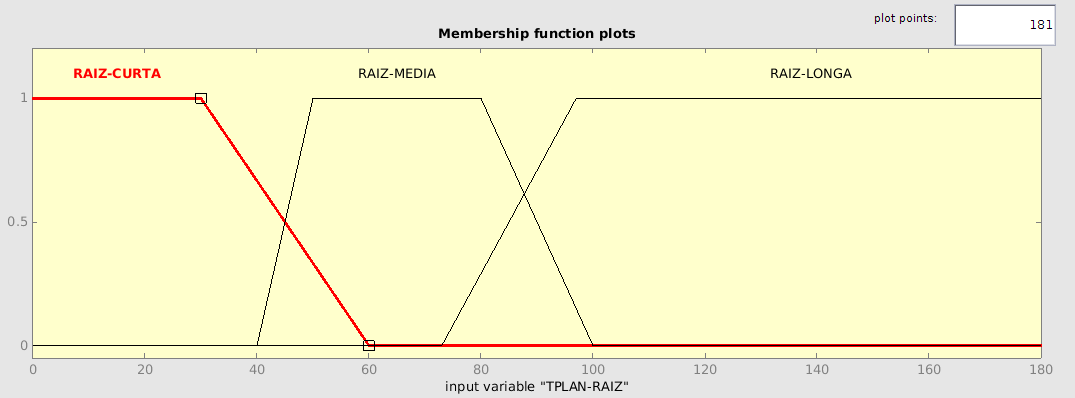
\includegraphics[width=1\linewidth]{Descricao/Imagens/TPLAN-RAIZ}
\caption{Tipo de raiz de cada planta}
\label{fig:TPLAN-RAIZ}
\end{figure}





\newpage
\subsubsection{TPLAN-DH}

\textbf{TPLAN-DH (TIPO-DE-PLANTA-DÉFICIT-HÍDRICO):} O deficit hídrico tolerável representa a tolerância das plantas à redução do conteúdo de água no solo, mantendo, ainda, sua capacidade de absorção de água.

\begin{table}[h!]
	\centering
	\rowcolors{3}{lightgray}{}
	\caption{Déficit hídrico tolerável para diferentes culturas}
	\label{tab:TPLAN-DH}
	\begin{tabular}{l c}
		\hline \hline
		\multirow{2}{*}{\textbf{Cultura}} & \textbf{Déficit Hídrico Tolerável (\%)} \\
		& \textbf{Gomes(1994)}                    \\
		\hline
		Alface                   & 35                             \\
		Cana-de-açúcar           & 15                             \\
		Feijão                   & 50                             \\
		Laranja                  & 35                             \\
		Melão                    & 20                             \\
		Milho                    & 40                             \\
		Morango                  & 10                             \\
		Tomate                   & 45                             \\
		\hline
	\end{tabular}
\end{table}

Exemplificando para o milho: a absorção de água pelas suas raízes fica comprometida
quando a retirada é maior que 40\% da capacidade de água disponível no solo.

\begin{figure}[h!]
\centering
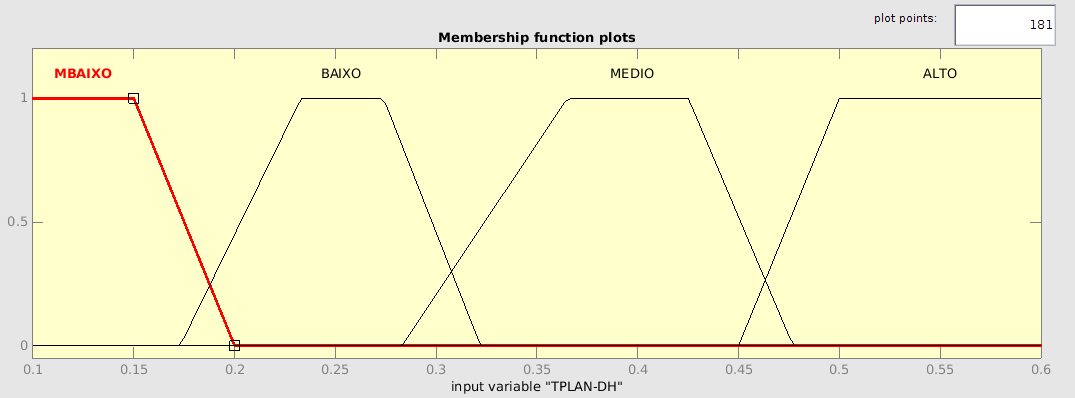
\includegraphics[width=1\linewidth]{Descricao/Imagens/TPLAN-DH}
\caption{Deficit hídrico da planta}
\label{fig:TPLAN-DH}
\end{figure}

\newpage
\subsubsection{ESTAG-C}

\textbf{ESTAG-C (ESTÁGIO-DE-CRESCIMENTO-DA-PLANTA):} Em geral, a planta tem um aumento progressivo de consumo hídrico até o período de floração e frutificação. A variável  \textbf{ESTAG-C}, assume diferentes valores de acordo com o tipo de cultura e a fase de crescimento da planta.

\begin{figure}[h!]
\centering
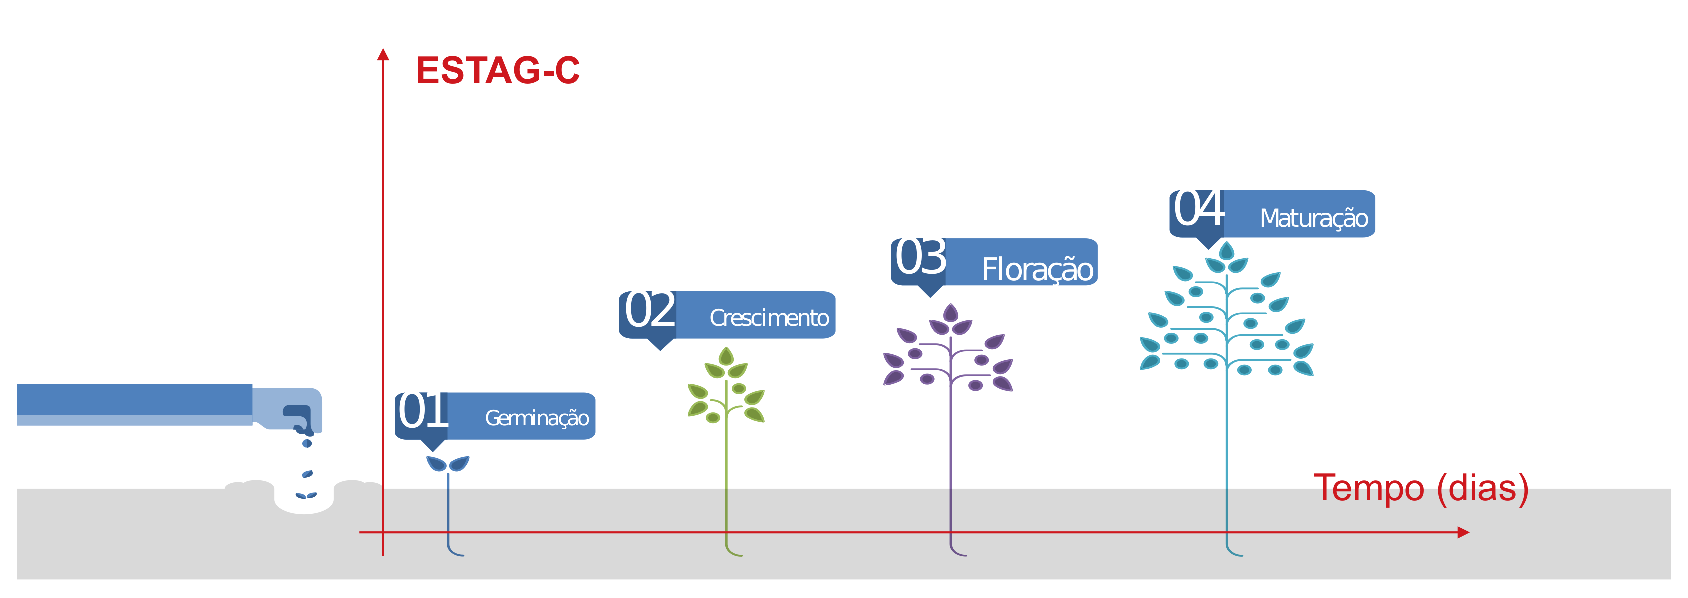
\includegraphics[width=1\linewidth]{Descricao/Imagens/estagio_de_crescimento}
\caption{}
\label{fig:estagio_de_crescimento}
\end{figure}



\begin{table}[h!]
	
	
	
	\centering
	\rowcolors{3}{lightgray}{}
	\caption{Valores médios do coeficiente de cultivo}
	\label{tab:ESTAG-C}
	\begin{tabular}{lcccc}
		\hline \hline
		\multirow{2}{*}{\textbf{Cultura}} & \textbf{Plantio-Germinação} & \textbf{Crescimento} & \textbf{Floração}  & \textbf{Maturação} \\
		& \textbf{Período 1}          & \textbf{Período 2}   & \textbf{Período 3} & \textbf{Período 4} \\
		\hline 
		Alface                   & 0,45               & 0,6         & 1         & 0,9       \\
		Cana-de-açúcar           & 0,5                & 1           & 1,1       & 0,65      \\
		Cítricos (ex. laranja)   & 0,65               & 0,7         & 1,7       & 0,65      \\
		Melão                    & 0,45               & 0,75        & 1         & 0,75      \\
		Milho                    & 0,4                & 0,8         & 1,15      & 1         \\
		Tomate                   & 0,45               & 0,75        & 1,15      & 0,8      \\
		\hline
	\end{tabular}
\end{table}


\begin{figure}[h!]
\centering
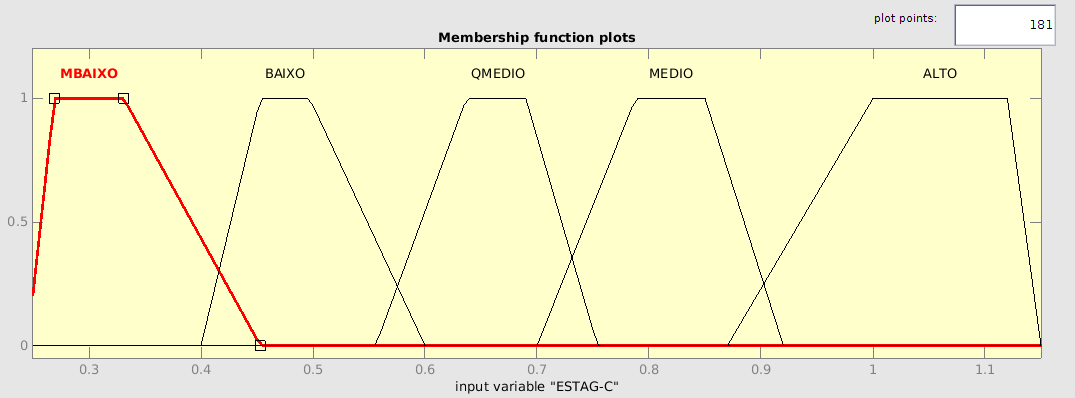
\includegraphics[width=1\linewidth]{Descricao/Imagens/ESTAG-C}
\caption{Estágio de crescimento da planta}
\label{fig:ESTAG-C}
\end{figure}


\subsubsection{TEMP}

\textbf{TEMP (TEMPERATURA):} Essa variável está associada à temperatura (em graus Celsius).

\begin{figure}[h!]
\centering
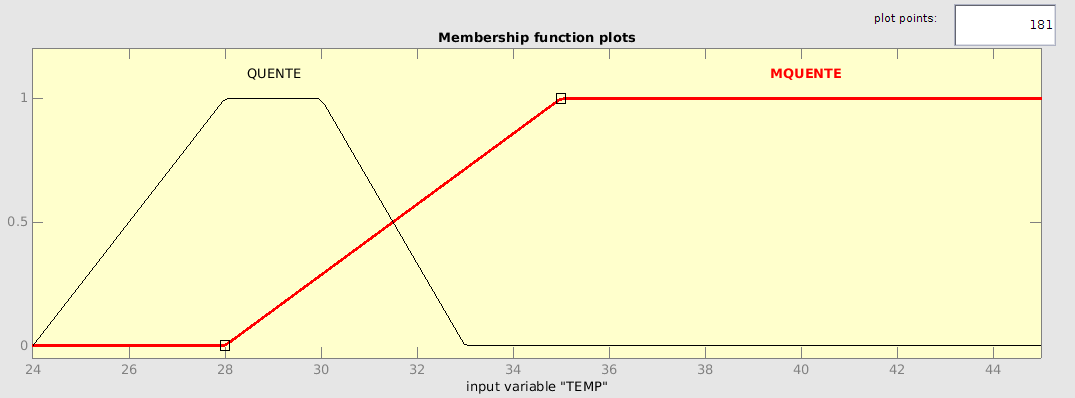
\includegraphics[width=1\linewidth]{Descricao/Imagens/TEMP}
\caption{Temperatura do ambiente na plantação}
\label{fig:TEMP}
\end{figure}



%\newpage
\subsection{Variáveis do Sistema - Variável de saída}

\subsubsection{UMD}

\textbf{UMD (UMIDADE-DO-SOLO):} Esta variável estabelece a referência de umidade que o solo deve possuir para o tipo de plantação em conjunto com todas as variáveis de entrada para um determinado momento da vida da planta (Germinação, Crescimento, Floração e Maturação).

\begin{figure}[h!]
\centering
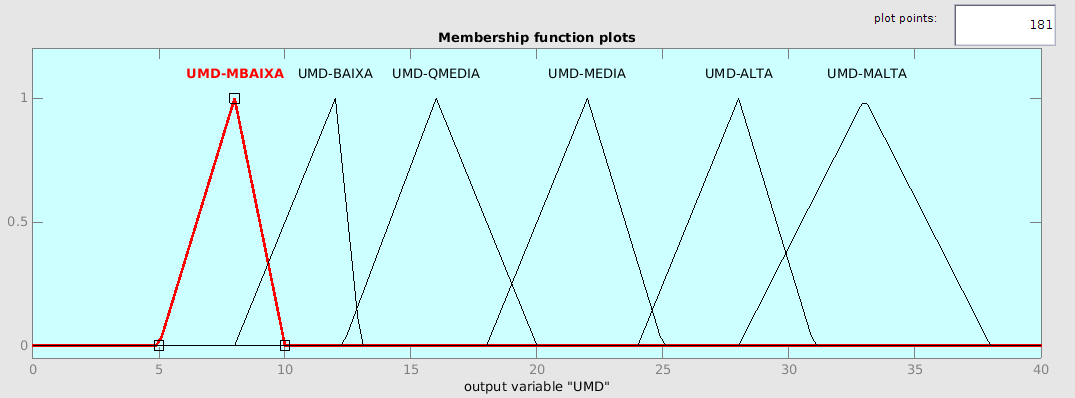
\includegraphics[width=1\linewidth]{Descricao/Imagens/UMD}
\caption{Umidade que se deseja para um determinado tipo de plantação}
\label{fig:UMD}
\end{figure}



